\chapter{Multi-view recalibration}
\label{cha:multi-view calibration}

\vspace*{-3ex}
The relation between the tools previously defined is provided here, explaining the way they work together in both the acquisition and estimation process.

This chapter is divided in three main sections: \textbf{acquisition}, \textbf{visualization} and \textbf{estimation}. Recall that the goal is to recalibration multiple cameras, using the PR2 as a real example, and focused in the estimation part.

\section{Overview}
\label{sec:estimation_overview}

In Figure \ref{fig:high_level_flow} a high level chart flow is presented: \textbf{1.} camera measurements are collected (checkerboard corners, as explained in section \ref{sec:acquisition}); \textbf{2.} then estimation process is optimizing a non-linear function in order to estimate the cameras poses; \textbf{3.} publishing the result to \texttt{/tf}.

\begin{figure}[!htbp]
 \centering
 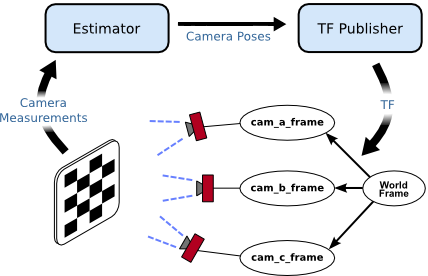
\includegraphics[width=0.5\textwidth]{images/high_level_flow_02.png}
 \caption{High level flow.}
 \label{fig:high_level_flow}
\end{figure}

\noindent
\textbf{Note}: point \textbf{3.} is optional. Since it was desired a visual feedback for the estimation process, it was necessary to considered this option from the beginning in the design. An alternative to \textbf{3.} is to save the result as a new and unique URDF for the particular robot it is being calibrated.



\subsection*{Preliminary: cameras in the PR2}

The PR2 has 6 cameras in its head:
\begin{itemize*}
 \item 2 narrow range. Topics: \texttt{wide\_right\_rect} and \texttt{wide\_left\_rect}.
 \item 2 wide range. Topics: \texttt{narrow\_right\_rect} and \texttt{narrow\_left\_rect}.
 \item 1 Kinect. Topic: \texttt{kinect\_head}.
 \item 1 High definition. Topic: \texttt{Prosilica\_rect}.
\end{itemize*}

\noindent
The initial camera configuration can be seen in Figure \ref{fig:pr2_cameras}, provided by the URDF. \textbf{Note}: this is the initialization and the information to be calibrated.
\begin{figure}[!htbp]
 \centering
 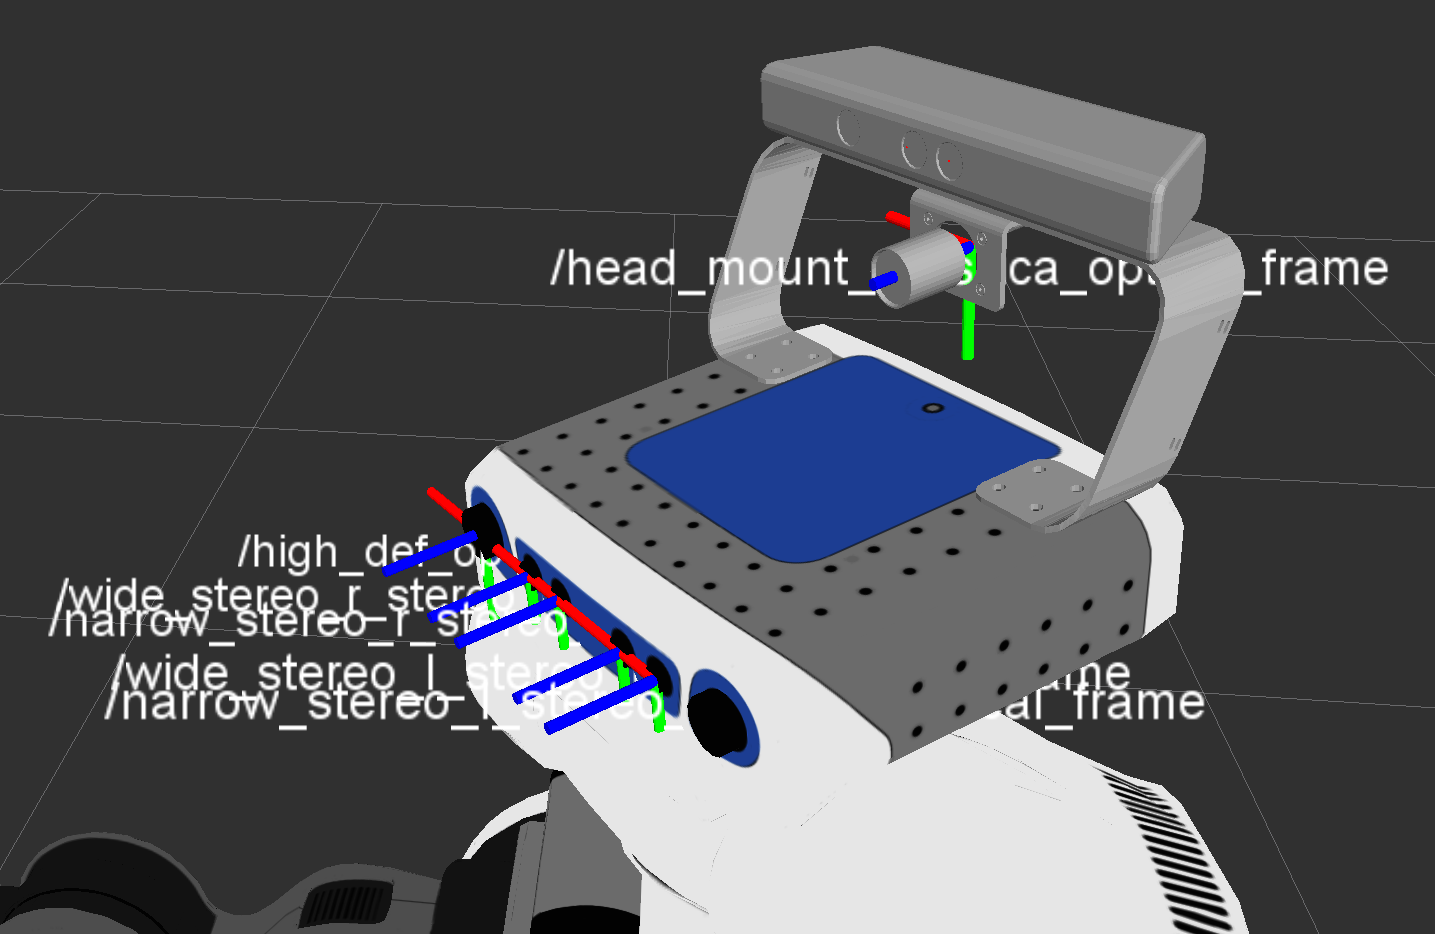
\includegraphics[width=0.55\textwidth]{images/screenshots/PR2_cameras.png}
 \caption{Coordinate system of all the cameras in the PR2 head.}
 \label{fig:pr2_cameras}
\end{figure}






\section{Acquisition process}
\label{sec:acquisition}

This is the \textit{point \textbf{1.}} in the overview (Figure \ref{fig:high_level_flow}). The acquisition part was already implemented, and a full description can be found in the paper  \cite{pr2_calibration_paper} and in the ROS tutorials for the PR2 calibration package.

% The thesis is focused in the estimation part but, in order to reach part, it is necessary first to do some comments regarding the process and
%
% % In the paper  and the ROS tutorials for the PR2 calibration package, the full description of the acquisition process will
% In this section will explain the acquisition process. It will explain


\subsection{Data collection}

In order to sufficiently constrain the non-linear optimization (see \cite{pr2_calibration_paper}), it is needed to collect a large amount of data, and manually collecting this calibration data can be tedious. By having the PR2 hold a checkerboard in its gripper (Figure~\ref{fig:pr2_holdind_cb}), a total of 30 checkerboard poses measurements are collected for each hand. Also, 4 samples of a \textbf{large checkerboard} that is far from the robot in order to help with far-field calibration (see Figure \ref{fig:data_collection01}). This data is saved in a ROS bag (section~\ref{sec:rosbag}) and posteriorly processed for the calibration package.

\noindent

\textbf{Notes}:
\begin{itemize*}
  \item It is important to mention at this point the 2D measurements are obtained from rectified images (section \ref{sec:rectification}). Therefore, working with distortion is happily avoided in the estimation process.
  \item It is assumed all cameras have been intrinsically calibrated in a previous stage.
\end{itemize*}


\begin{figure}[!htbp]
  \centering
  \raisebox{2ex}{
    \subfigure
    {
      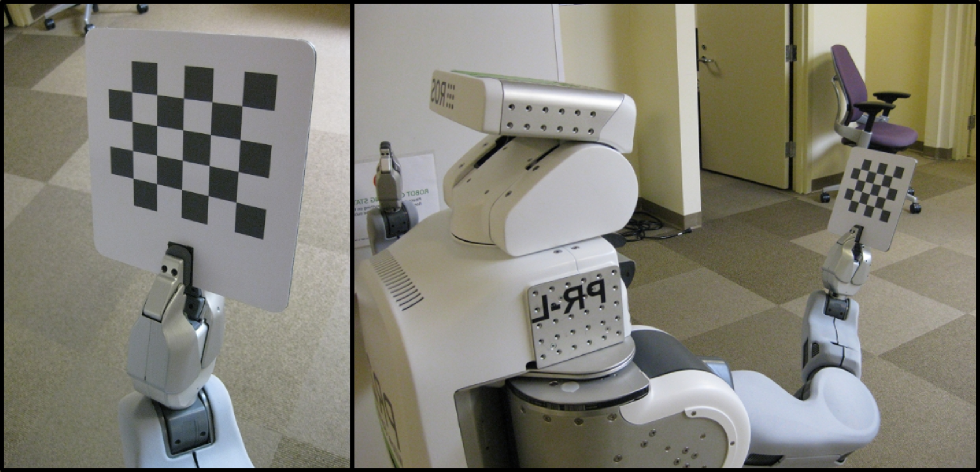
\includegraphics[width=0.5\textwidth]{images/pr2_holdind_cb.png}
    }
  }
  \subfigure
  {
    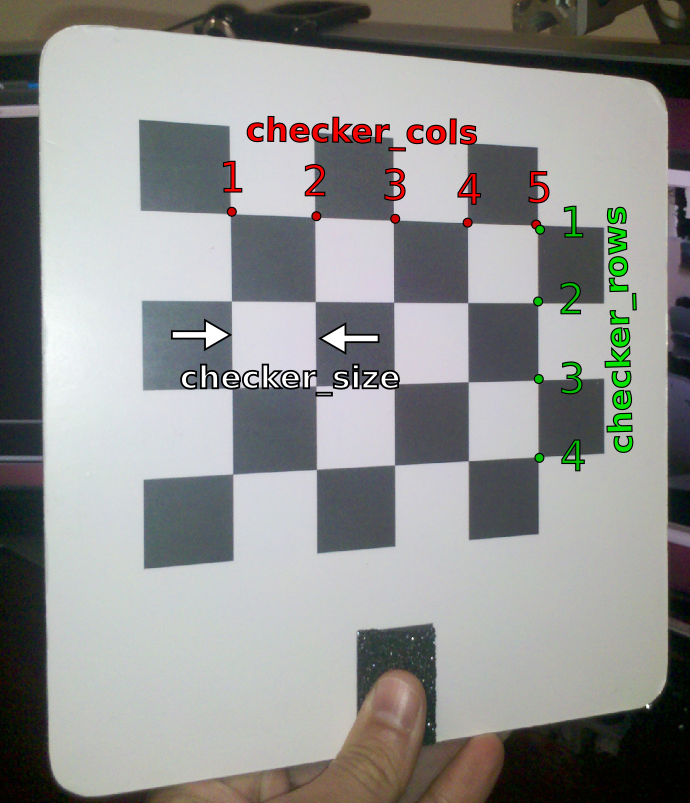
\includegraphics[width=0.25\textwidth]{images/checkerboard01.png}
  }
  \caption{The PR2 holding a checkerboard pattern.}
 \label{fig:pr2_holdind_cb}
\end{figure}


\begin{figure}[!htbp]
 \centering
 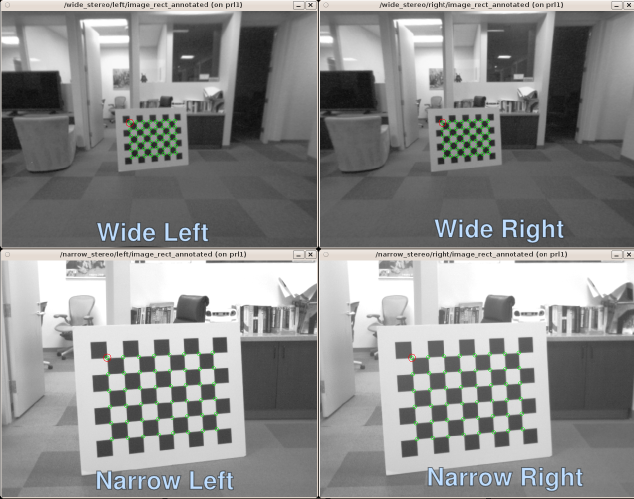
\includegraphics[width=0.7\textwidth]{images/data_collection01.png}
 \caption{Example of \textit{one} sample from 4 different view, using the large checkerboard.}
 \label{fig:data_collection01}
\end{figure}




\section{Visualization}
\label{sec:visualization}

This is the \textit{point \textbf{3.}} in the overview (Figure \ref{fig:high_level_flow}). This part is optional, but it was crucial to understand what was happening and to debug problems and solutions.

Even though publishing to /tf is not difficult to do, it has been time consuming and more details will be given in chapter \ref{cha:implementation}. %, where implementation details are given\footnote{Publish to /tf is mentioned here to be consistent with the overview.}.

For now, let's us concentrate in 3D points visualization, more precisely RViz Markers.

\subsection{Visual Markers}
\label{sec:visual_markers}

Since checkerboards are seen from multiple views, an idea to check if the system is calibrated is to overlap the 3D obtained from individuals cameras using solvePnP, described in section \ref{sec:solvePnP}. Two examples can be seen in Figure \ref{fig:visual_markers}. Different colors have been used for different cameras.

\begin{figure}[!htbp]
  \centering
  \subfigure[Checkerboard in hand.]{
    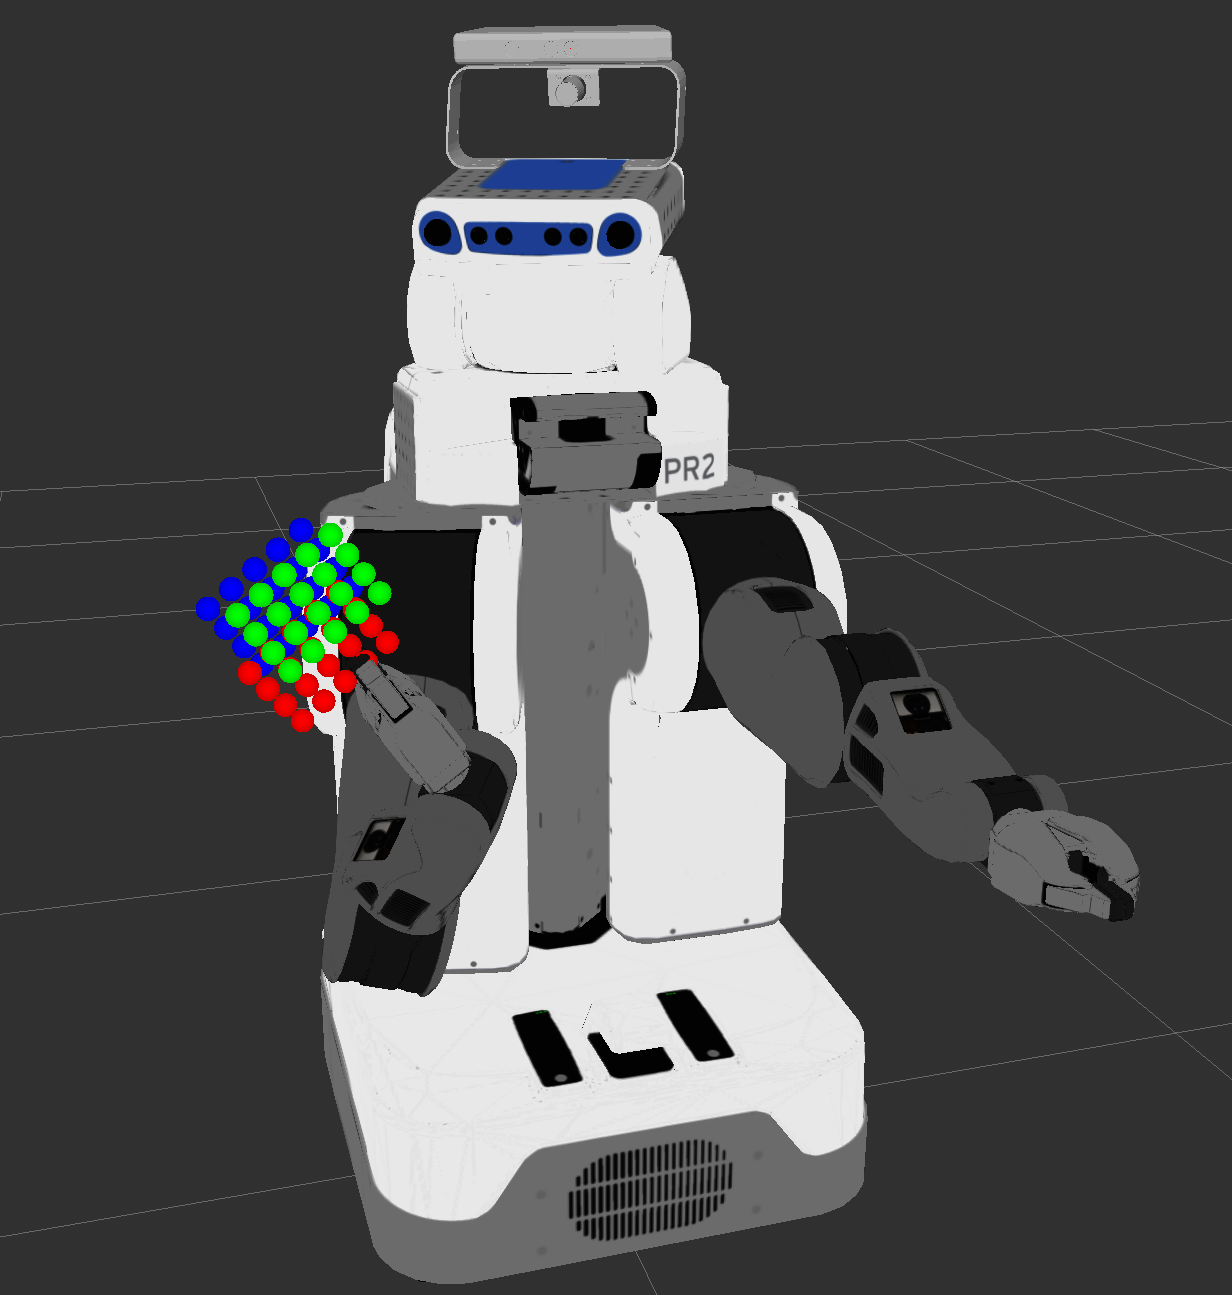
\includegraphics[height=0.35\textheight]{images/screenshots/uncalib10_1.png}
  }
  \subfigure[Checkerboard free in the world.]{
    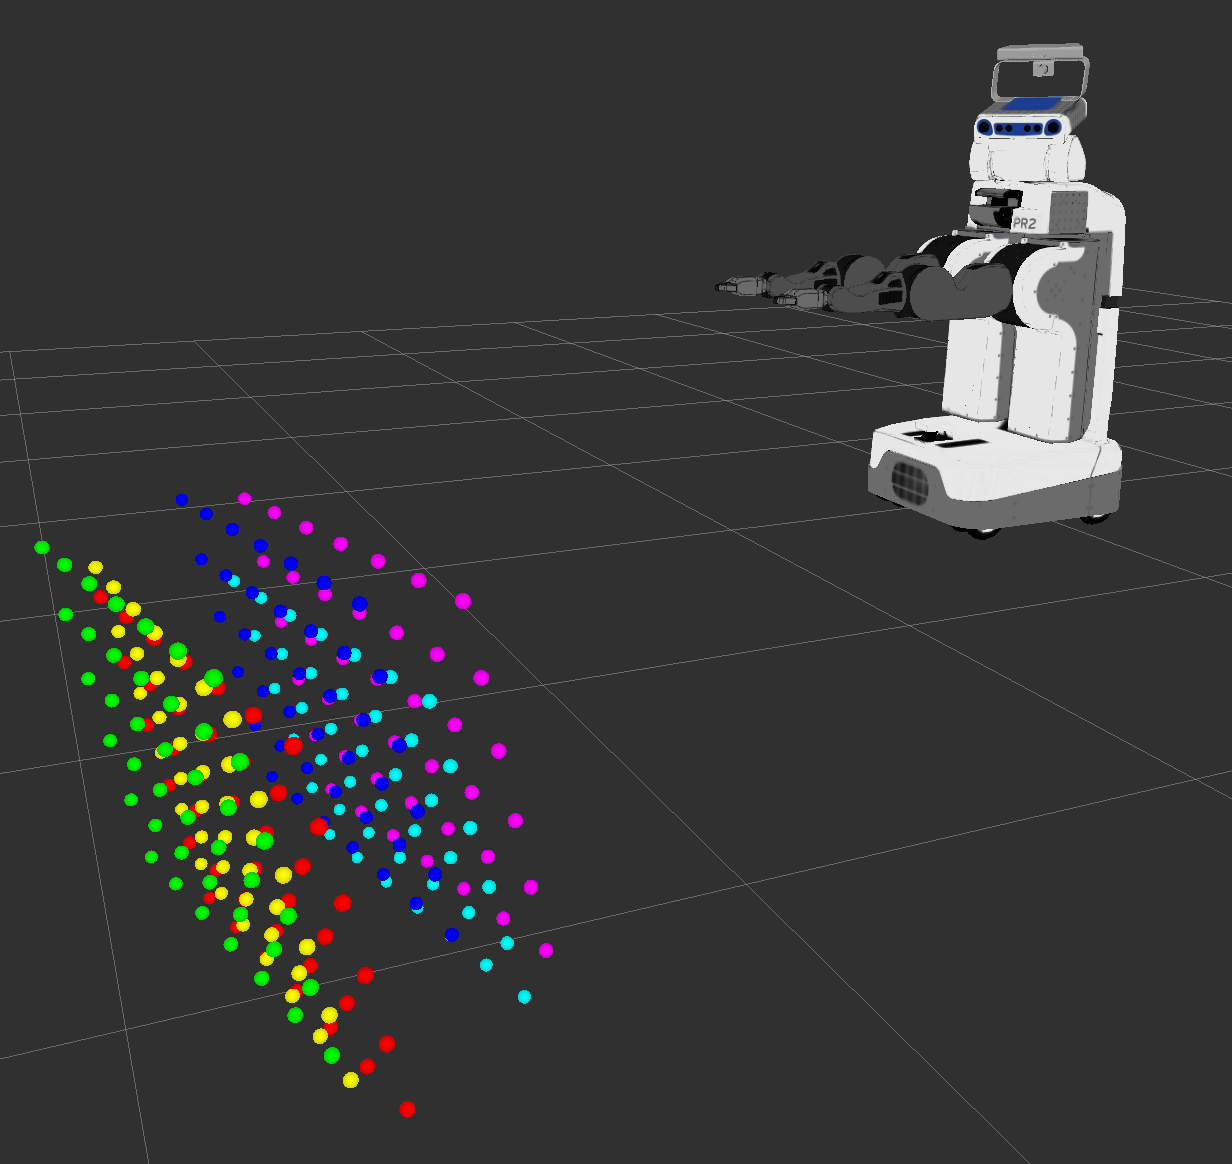
\includegraphics[height=0.35\textheight]{images/screenshots/uncalib03_1.png}
  }
  \caption{solvePnP results for the all the cameras (same checkerboard).}
  \label{fig:visual_markers}
\end{figure}

\noindent
\textbf{Note:} this is not the best approach to get 3D points since they are obtained from measurements of individual cameras. It is used here for a quick comparison, in order to see how bad the calibration is. A superior method is to use all the cameras measurements minimizing an \textit{algebraical error} (linear), the n-view triangulation method (section \ref{sec:nview_triangulation}); and followed by a \textit{geometrical error} minimization (non-linear), the re-projection error. It is superior because it is optimal in the \textbf{maximum likelihood} sense.

\section{Estimation process}
\label{sec:estimation}

This is the \textit{point \textbf{2.}} in the overview (Figure \ref{fig:high_level_flow}).
The estimation process is divided in turn in three stages: \textbf{initialization}, actual \textbf{optimization} and \textbf{updating} URDF robot model with the results (see Figure \ref{fig:optimization}).

\begin{figure}[!htbp]
 \centering
 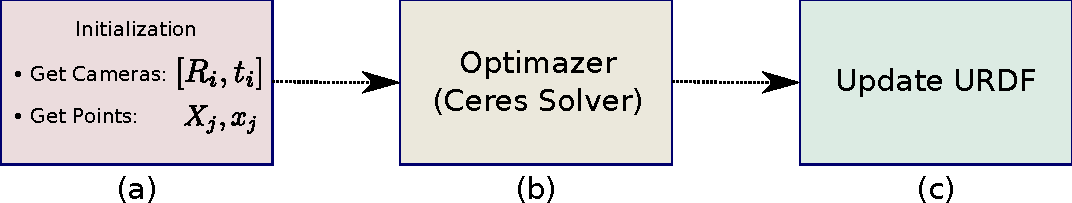
\includegraphics[width=0.7\textwidth]{images/optimization.pdf}
 \caption{Estimation process.}
 \label{fig:optimization}
\end{figure}

% Needing to estimate relative poses of several cameras or many poses of a single moving camera is a somewaht common problem. It is often solve by jointly estimating the set of camera poses along with 3D features that are detected by some set of cameras. This approach is called bundle adjustment \cite{BA}.
%
% We have in condition now explain the estimation process, all the needed components have been explained.


\subsection{Initialization}

\subsubsection*{Get cameras}

An \textbf{initial configuration} of the cameras is given by the URDF, it comes from the robot design.

Since PR2 head moves in the data collection, the camera poses change with respect to the robot coordinate system in each calibration step, depending of the angles joints. Them, \textbf{forward kinematics} is needed and KDL (section \ref{sec:KDL}) is extremely useful here.
\textbf{Note}: even though the robot moves, the relative position of the cameras does not change, it is a rigid relationship between them since they are all located in head which is a whole entity.

\begin{figure}[!htbp]
 \centering
 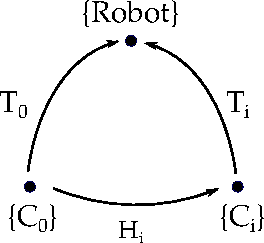
\includegraphics[width=0.3\textwidth]{images/initialization.pdf}
 \caption{Relative transformations.}
 \label{fig:initialization}
\end{figure}

\noindent
In order to understand Figure \ref{fig:initialization}, some terms are introduced below:
\begin{itemize*}
 \item[-] \{\textbf{Robot}\}: robot coordinate system. It is the root of the URDF tree, usually called \texttt{base\_footprint} link.

 \item[-]  \{$\mathbf{C_i}$\}: camera coordinate system $i$. The \textit{reference camera} is $C_0$.

 \item[-]  \{$\mathbf{T_i}$\}: transformation from  \{$\mathbf{C_i}$\} to \{\textbf{Robot}\}.

 \item[-] \{$\mathbf{H_i}$\}: transformation from  \{$\mathbf{C_0}$\} to  \{$\mathbf{C_i}$\}. It is the relative position between them, from rotation and translation matrices are obtained.
\end{itemize*}

% \noindent
Then,
\begin{equation}
 H_i = T_i^{-1} \, T_0
\end{equation}

rotation $R_i$ and translation $t_i$ of the camera $i$ can be extracted from $H_i$,
\begin{equation}
 H_i = \begin{pmatrix}
        R_i & t_i \\
        0   & 1
        \end{pmatrix}
\end{equation}

\subsubsection*{Get points}

Now, 3D points should be obtained from the measurements as an initialization. Two initialization are possibles:
\begin{itemize*}
 \item using \textbf{solvePnP} (section \ref{sec:solvePnP}) in the reference camera, 3D points will minimize re-projection error in the first camera. This is not an optimal initialization, as it is explained in the end of section \ref{sec:visualization},

 \item using \textbf{n-view triangulation} (section \ref{sec:nview_triangulation}): by the moment of writing the thesis, this part is considered as ``\textit{work in progress}'', therefore results of this initialization are not provided, more details of the problems encountered are explained in the implementation chapter \ref{cha:implementation}. Note: it is a natural extension of the triangulation method, which minimize an algebraical error. This could be a better initialization for the structure in comparison with the previous one.
\end{itemize*}



\subsubsection*{Get projection matrices}

As it stated in section \ref{sec:BA}, BA takes \textbf{measurements}, \textbf{3D Points} (structure) and \textbf{projection matrices}~$P_i$. The last step needed here is to multiply $[R_i ~~ t_i]$ by $K_i$ (camera intrinsic matrix), and it is assumed to have this information. Then,
\[
 P_i = K_i \, [R_i ~~ t_i]
\]




\subsection{Per view optimization}

In order to test the system before going to the complete optimization (optimizing the parameters with data in all views), a ``local'' per view optimization (only one checkerboard sample) was performed to see if the process was going in the right path. This previous stage before using all the data was important to find errors.

TODO... Move to implementation chapter!!



\subsection{Optimizer}

This part will be considered in the implementation chapter (section \ref{sec:ceres_impl}).


\subsection{Update URDF}

TODO....



------------------


\subsection{Results}
\label{sec:results}

In this section, a visual comparison is given. First, result before and after optimization process are compared visually using solvePnP as is described in section \ref{sec:visual_markers}. Second, a quantitative comparison of the optimization process output is provided.

\subsubsection{Visual comparison}

Only two of a total of 64 checkerboard samples are shown here: checkerboard in hand in Figure \ref{fig:cal_hand}, and checkerboard free in the world in Figure \ref{fig:cal_free}. It is possible to appreciate that after the optimization process the checkerboards are more close each others, indicating it is a better calibration has been obtained, next section gives a more exhaustive comparison of the estimation process results.
% it does not mean it is a good one.
%

\begin{figure}[!htbp]
 \centering
   \subfigure[Before estimation.]
   {
      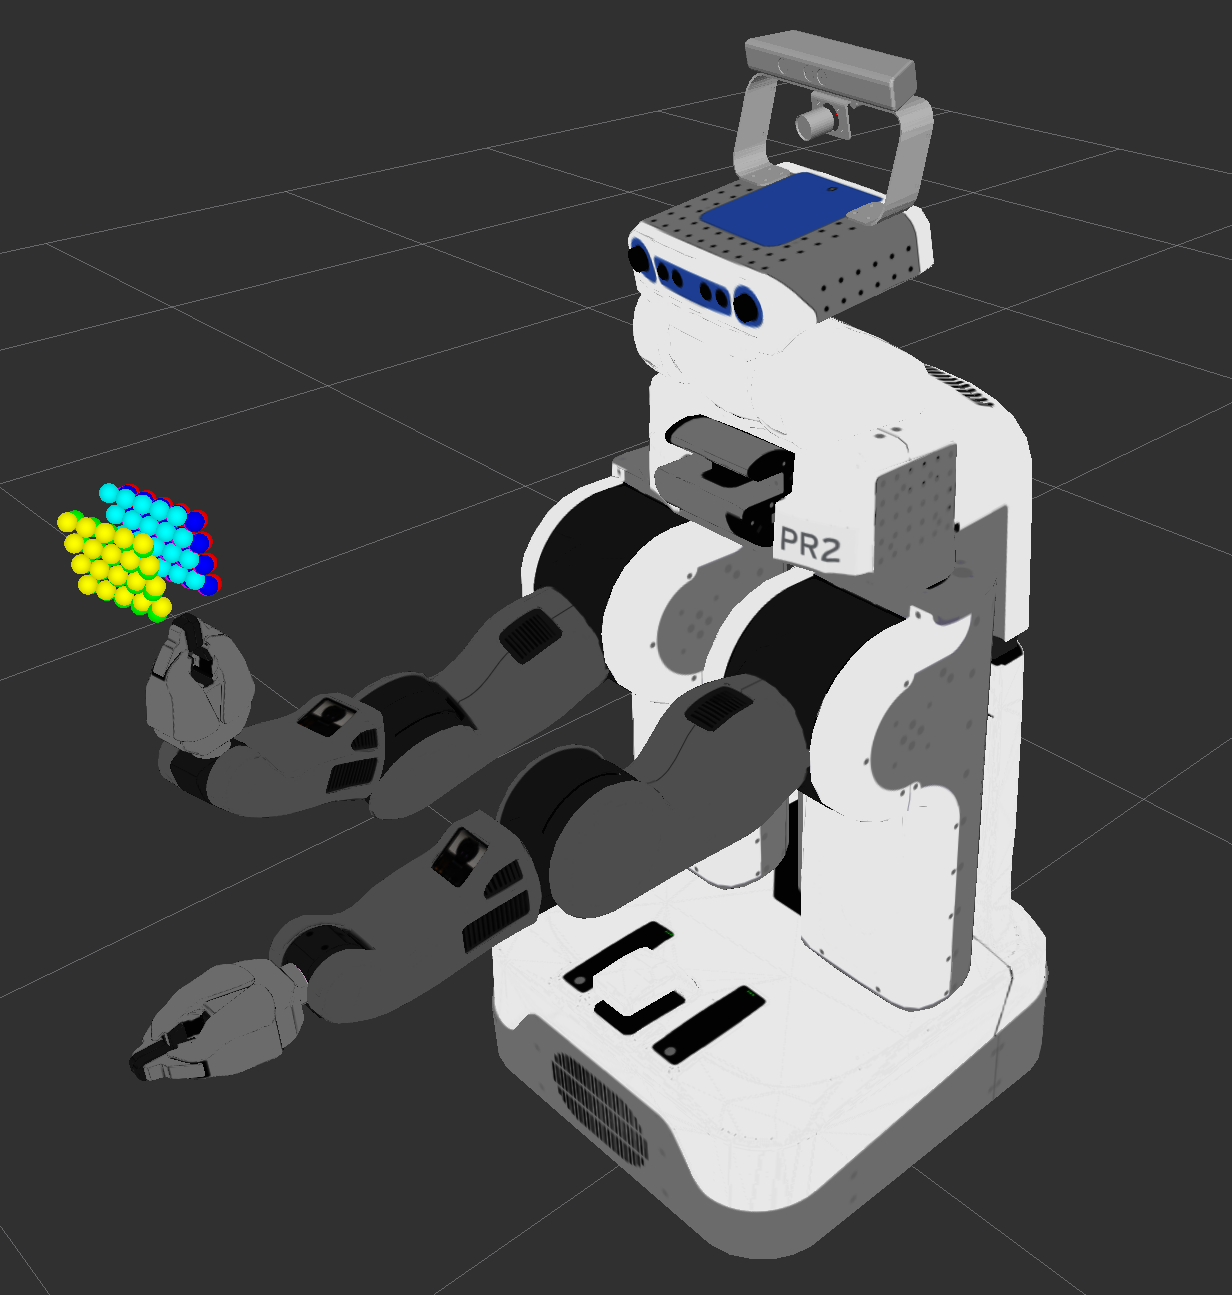
\includegraphics[height=0.25\textheight]{images/screenshots/uncalib08_1.png}
   }
   \subfigure[After estimation.]
   {
      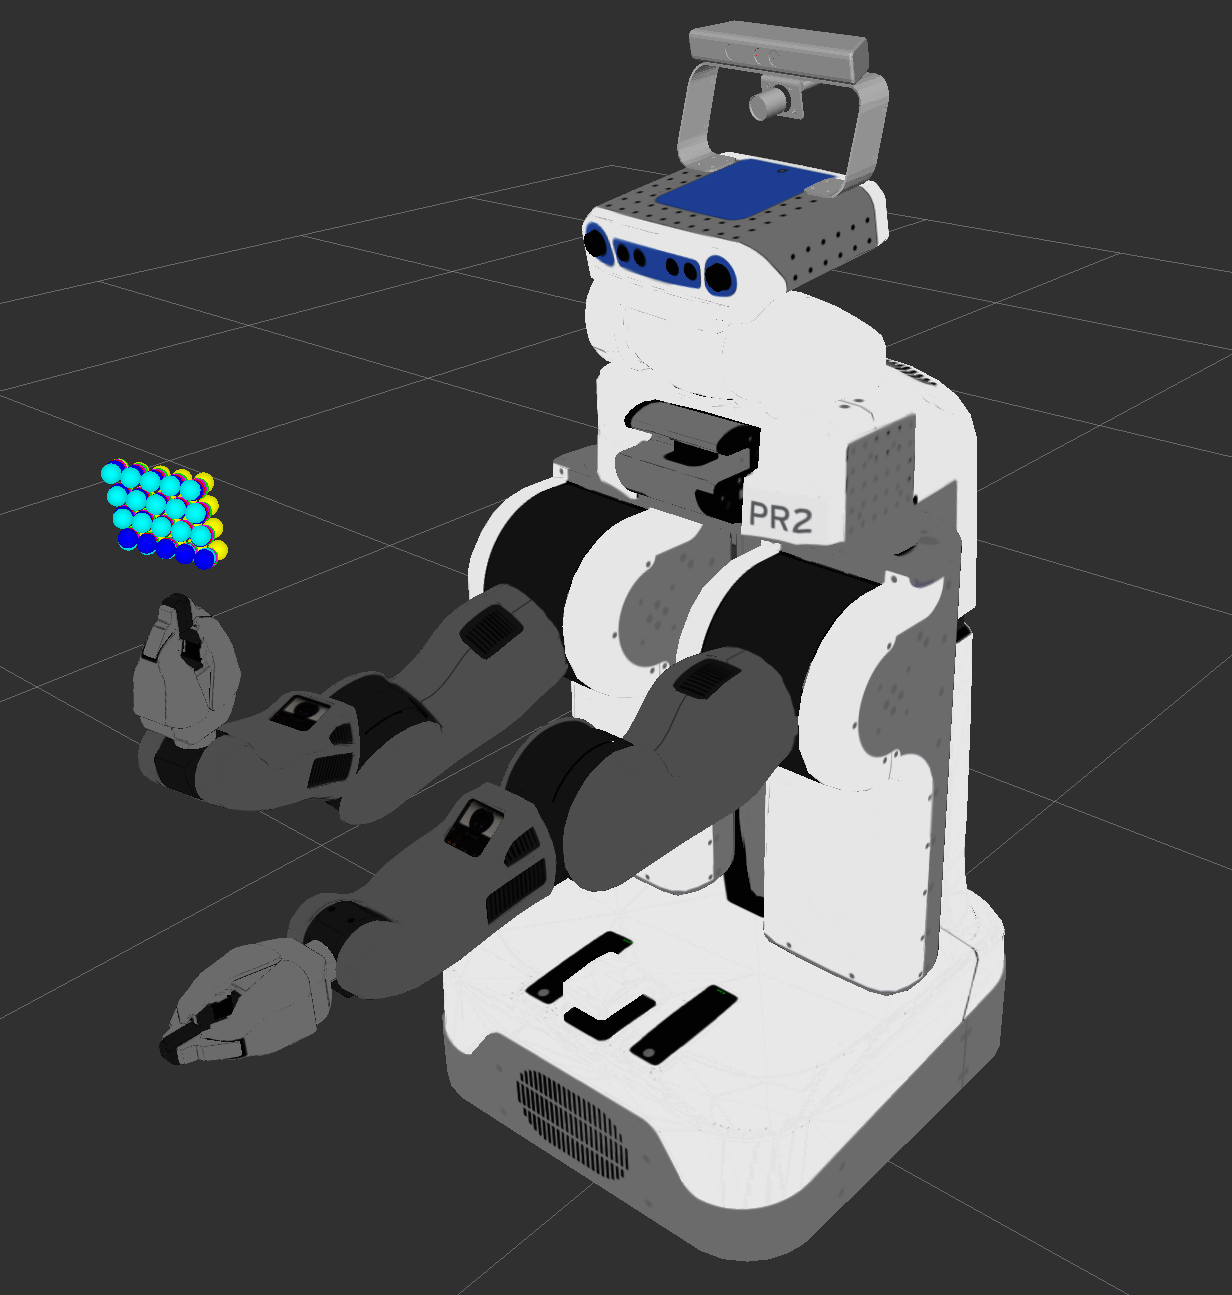
\includegraphics[height=0.25\textheight]{images/screenshots/calib08_1.png}
   }
 \caption{Checkerboard in hand.}
 \label{fig:cal_hand}
\end{figure}


\begin{figure}[!htbp]
 \centering
   \subfigure[Before estimation.]
   {
      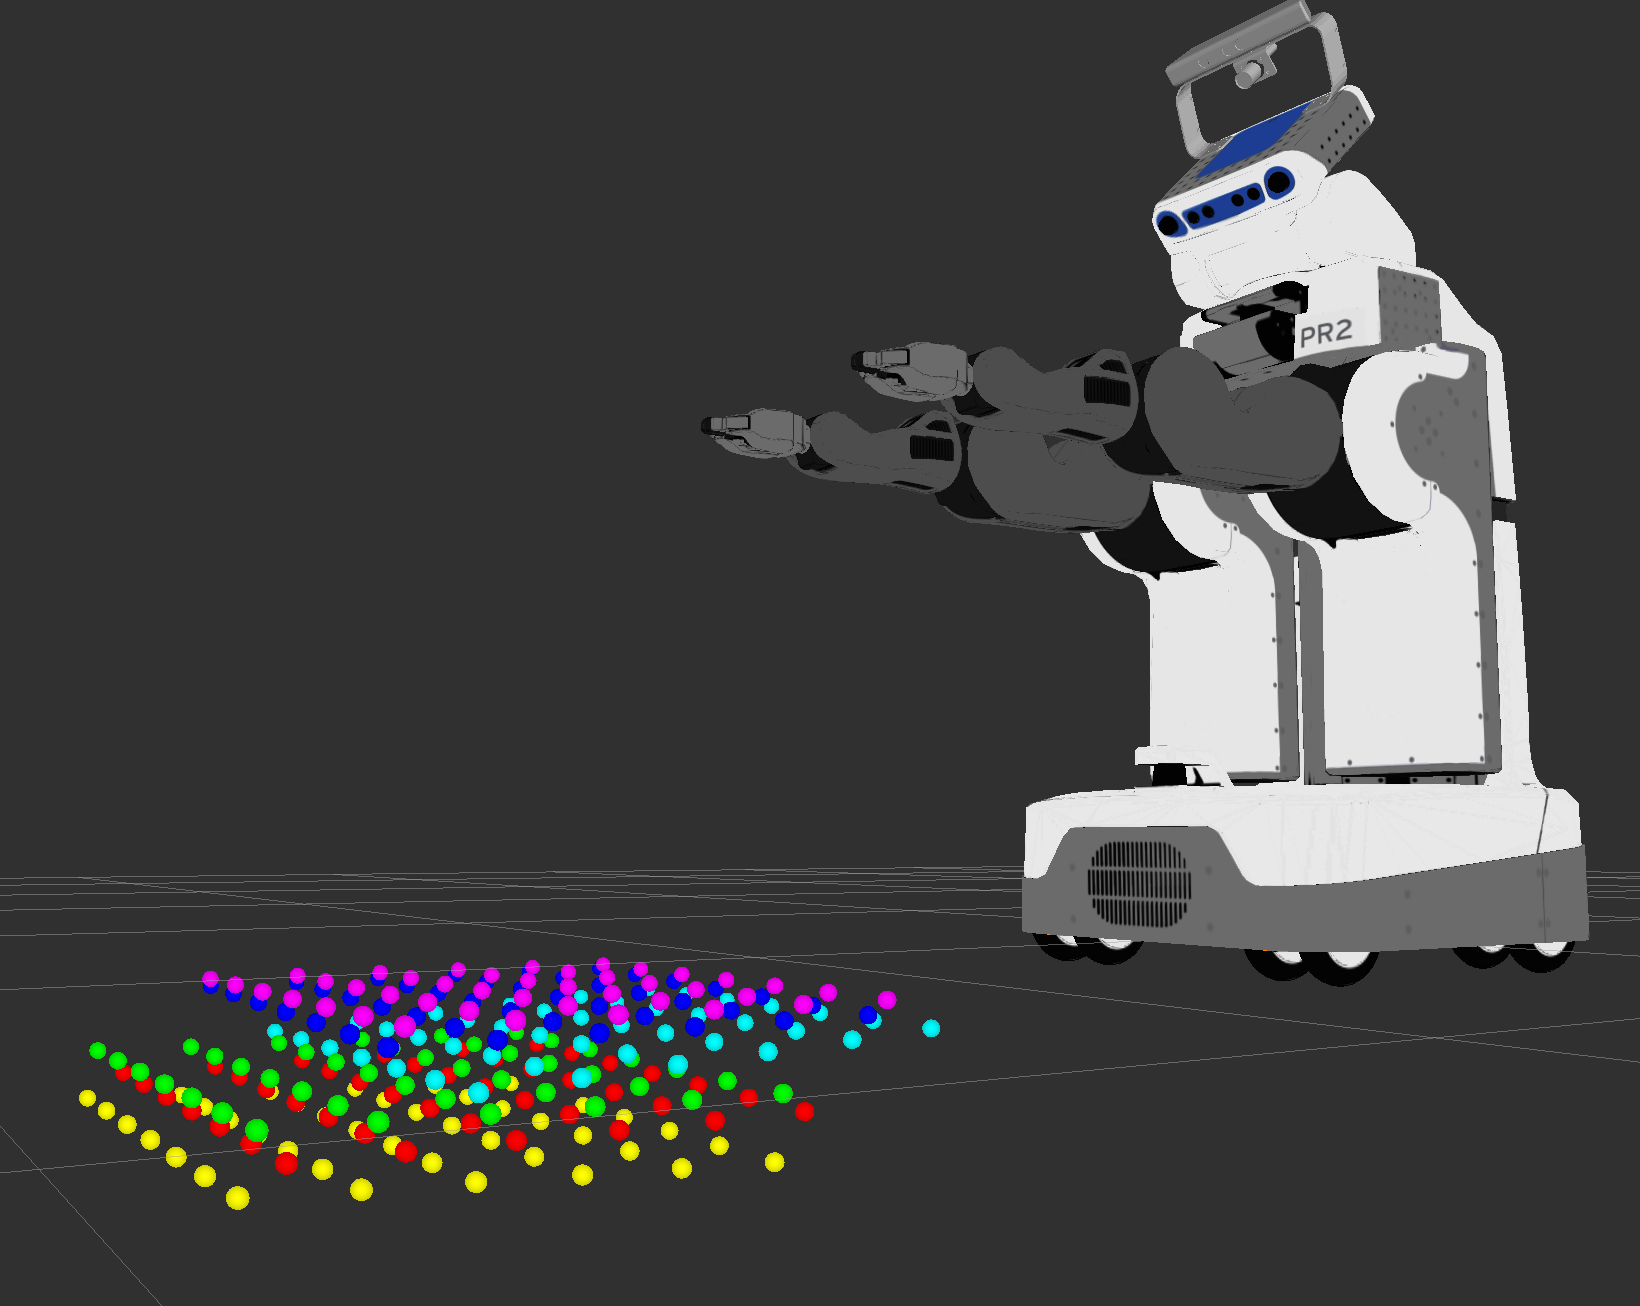
\includegraphics[height=0.25\textheight]{images/screenshots/uncal01_1.png}
   }
   \subfigure[After estimation.]
   {
      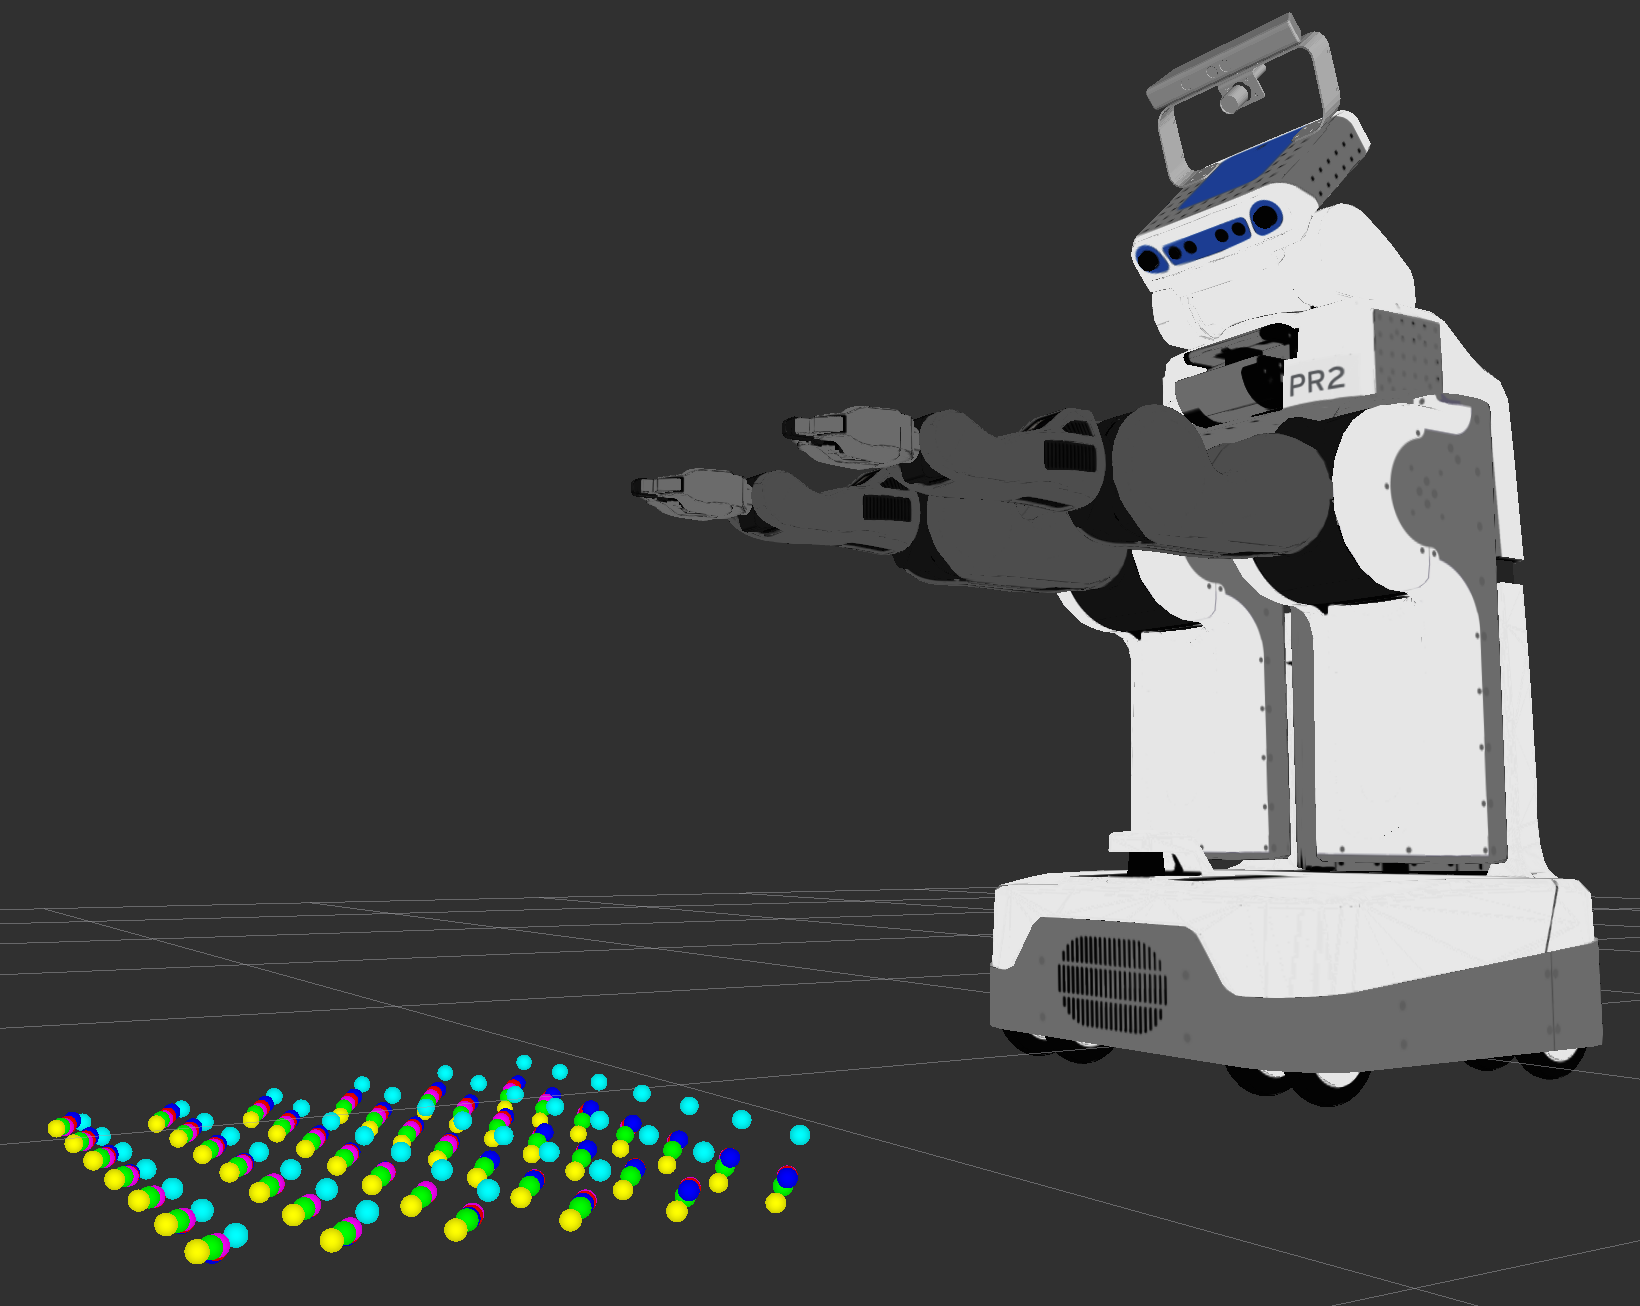
\includegraphics[height=0.25\textheight]{images/screenshots/cal01_1.png}
   }
 \caption{Checkerboard free in the world.}
 \label{fig:cal_free}
\end{figure}

\textbf{Note}: one of the camera does not show a good result (specially in Figure \ref{fig:cal_free}), corresponded to the prosilica camera, and a probable factor of this problem will be mentioned in the next section.


\subsubsection{Quantitative results}

As is mentioned above, the only finished implementation is the one which use solvePnP to find 3D points in the first camera (reference camera), and using those points as initialization for the structure. It is not an optimal solution and arise with a bias on the reference camera (\texttt{narrow\_left\_rect}): it has an excellent re-projection for the first camera in comparison with rest, as is perceived in Figure \ref{fig:boxplot_stats}.
% \begin{figure}[!htbp]
%  \centering
%  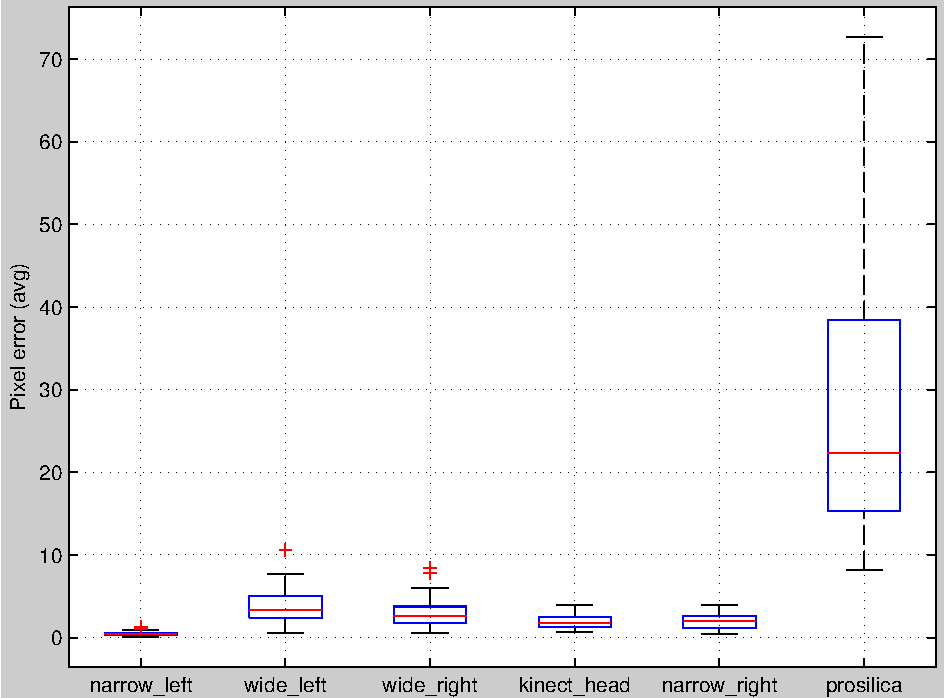
\includegraphics[width=0.35\textwidth]{images/boxplot_stats.pdf}
%  \caption{Visible bias in the first camera}
%  \label{fig:boxplot_stats}
% \end{figure}

\begin{figure}[!htbp]
 \centering
   \subfigure[With \texttt{prosilica} camera]
   {
      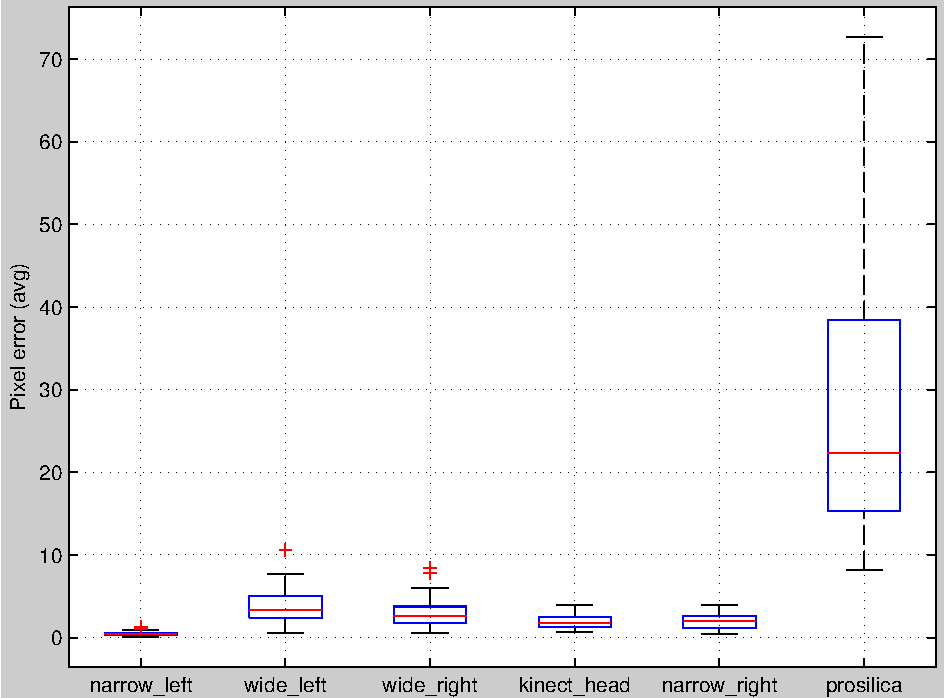
\includegraphics[height=0.25\textheight]{images/boxplot_stats.pdf}
      \label{fig:boxplot_stats}
   }
   \subfigure[Without \texttt{prosilica} camera]
   {
      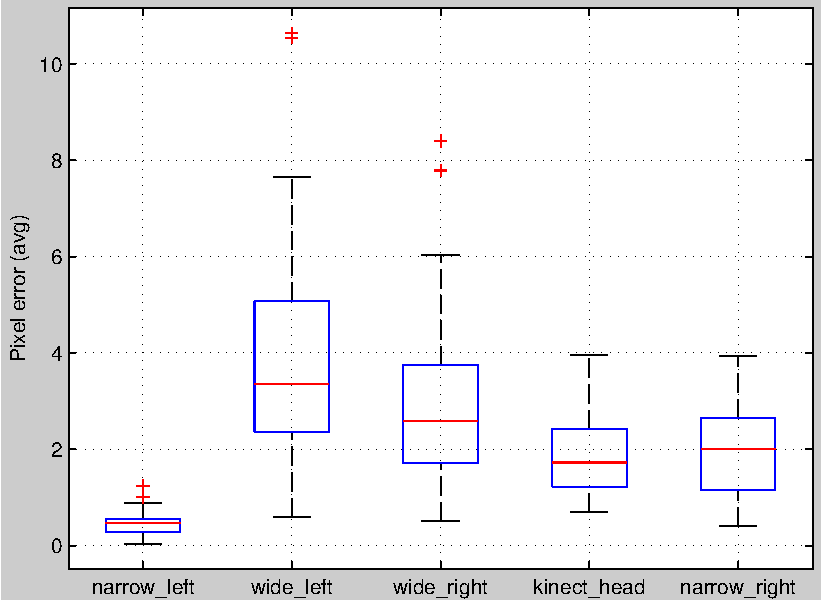
\includegraphics[height=0.25\textheight]{images/boxplot_stats_without_prosilica.pdf}
      \label{fig:boxplot_stats_without_prosilica}
   }
 \caption{Visible bias on first camera (with and without \texttt{prosilica} camera)}
%  \label{fig:boxplot_stats}
\end{figure}

In addition, it is possible to observe the \texttt{prosilica} camera has a bigger error than the remaining cameras. A wrong intrinsic calibration could be the reason. In order to determine if the bias was produced for this camera, same comparison has been repeated without taking into account the \texttt{prosilica} camera in the estimation process (Figure \ref{fig:boxplot_stats_without_prosilica}). Even though the global re-projection improves in this case, the bias continues on the first camera.




A visible comparison of this bias can been noted in Figure \ref{fig:reprojection}, where reprojected points after optimization are plot for two cameras: \texttt{wide\_left\_rect} and \texttt{narrow\_left\_rect} camera.
\begin{figure}[!htbp]
  \centering
    \subfigure[\texttt{wide\_left\_rect} camera]
    {
      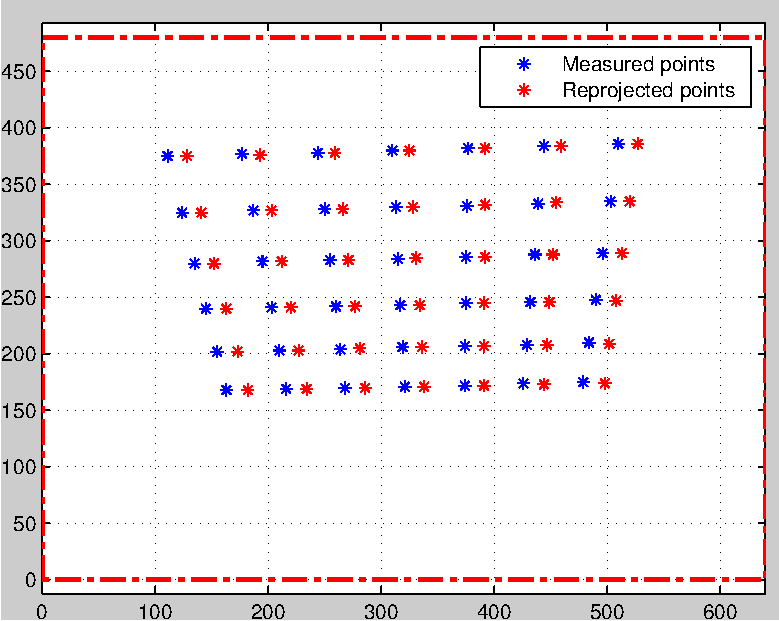
\includegraphics[width=0.45\textwidth]{images/reprojection02.pdf}
      \label{reprojection02}
    }
  \subfigure[\texttt{narrow\_left\_rect} camera (reference cam.)]
  {
    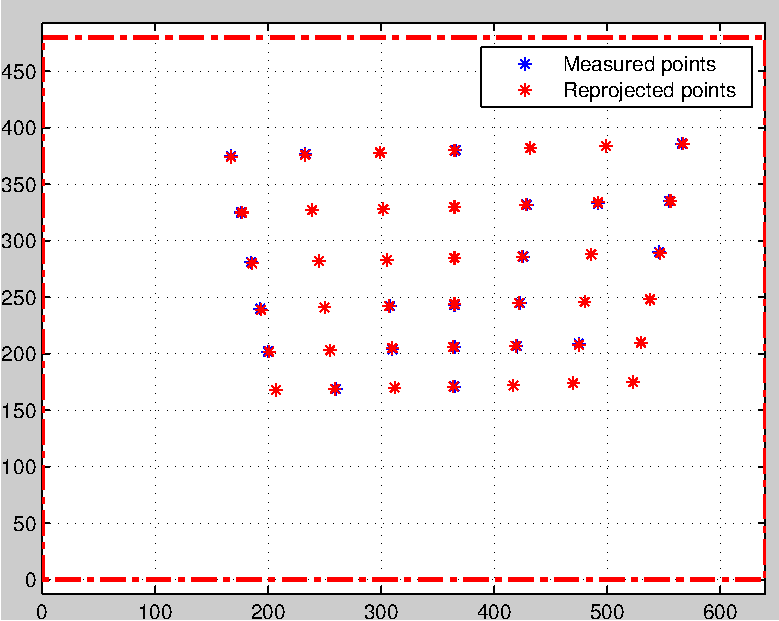
\includegraphics[width=0.45\textwidth]{images/reprojection01.pdf}
    \label{reprojection01}
  }
  \caption{Re-projection error after optimization}
  \label{fig:reprojection}
\end{figure}



More statistics (median, mean and standard deviation) can be observed in Figure \ref{fig:stats}.
\begin{figure}[!htbp]
 \centering
 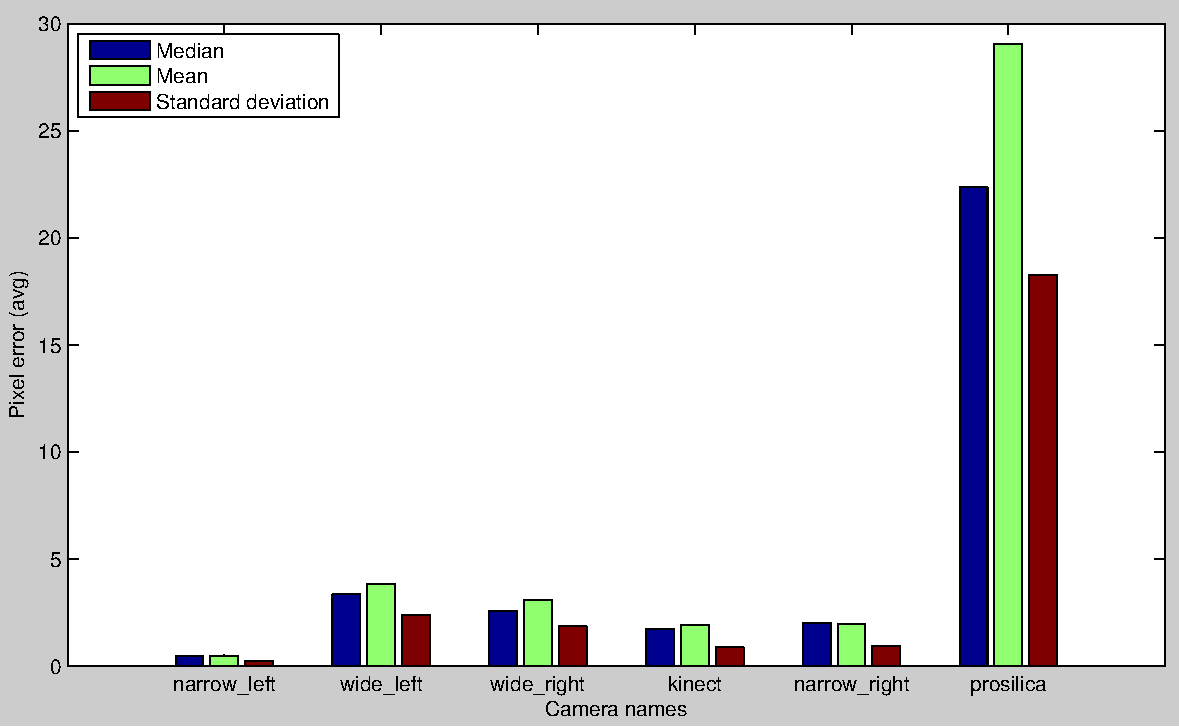
\includegraphics[width=0.65\textwidth]{images/stats.pdf}
 \caption{Median, mean, std after optimization}
 \label{fig:stats}
\end{figure}


Speed was not a priority goal of this project, but worth to mention that Ceres Solver takes few seconds to compute the result and less than 50 iteration to converge.


